\documentclass{elsarticle}

% Mathematics
\usepackage{amsmath}
\usepackage{amssymb}
\usepackage{amsthm}
\usepackage{fullpage}

% Figures
\usepackage{graphicx}

% Algorithms
\usepackage{algorithm}
\usepackage{algpseudocode}
\algrenewcommand\Require{\hspace*{\algorithmicindent} \textbf{Input}:  }
\algrenewcommand\Ensure{\hspace*{\algorithmicindent} \textbf{Output}:  }

% Text and formatting
\usepackage{xcolor}
\usepackage{soul}
\usepackage{booktabs}

% References
\usepackage{natbib}

\journal{Computer Methods in Applied Mechanics and Engineering}

\begin{document}

\begin{frontmatter}

\title{Adaptive Delayed-Acceptance MCMC with posterior guided active learning}

\author[polimi-mox, pasteur]{Filippo Zacchei}
\author[polimi-dica]{Attilio Frangi}
\author[polimi-mox]{Andrea Manzoni}

\address[polimi-mox]{Politecnico di Milano, MOX -- Department of Mathematics,
P.za Leonardo da Vinci 32, 20133 Milano, Italy}

\address[polimi-dica]{Politecnico di Milano, Department of Civil and Environmental Engineering,
P.za Leonardo da Vinci 32, 20133 Milano, Italy}

\address[pasteur]{Pasteur Labs, Brooklyn, NY, USA}


\begin{abstract}
Inverse uncertainty quantification tasks, such as Bayesian parameter estimation,
are computationally demanding when the forward model is a physics-based
numerical solver. In particular, for systems governed by partial differential
equations, full-order discretizations, such as finite elements or finite
volumes, make conventional Markov chain Monte Carlo sampling prohibitively
expensive, due to the large number of forward evaluations required. Surrogate
models can reduce this cost, but their effectiveness is often limited by the
offline generation of high-fidelity training data. A natural remedy is to
construct the surrogate online, concurrently with posterior sampling, so that
training points concentrate in posterior-relevant regions.
We propose an adaptive delayed-acceptance MCMC method in which a surrogate
combining proper orthogonal decomposition and Gaussian process regression
provides a cheap first-stage approximation of the likelihood. The surrogate is
refined sequentially during sampling, and its predictive uncertainty is used to
decide when a high-fidelity model evaluation is required. The delayed-acceptance
construction preserves the high-fidelity posterior as the invariant target
distribution, while reducing the number of expensive solver calls.
Numerical experiments on two benchmark inverse problems, namely a
mass-spring-damper system and an incompressible Navier--Stokes problem with
variable geometry, show that the proposed strategy provides accurate posterior
estimates with improved computational efficiency compared with standard
single-stage MCMC and non-adaptive surrogate schemes.
\end{abstract}

\begin{keyword}
Bayesian inverse problems \sep Markov chain Monte Carlo
\sep Gaussian process regression \sep Proper orthogonal decomposition \sep
Surrogate modelling
\end{keyword}

\end{frontmatter}

\section{Introduction}

Parameter estimation is central to predictive modelling in engineering \cite{BK19}, where unknown physical or constitutive quantities must be inferred from indirect and often noisy observations. Reliable estimates are essential in applications such as fluid mechanics  \cite{CDRS09}, climate modelling \cite{SLST17}, structural engineering \cite{GR22}, and micro-scale devices \cite{ZRGFM24}, where parameter uncertainty can affect prediction quality, design decisions, and operational safety. Although high-fidelity numerical solvers have substantially improved the simulation of such systems, the underlying models are often governed by Partial Differential Equations (PDEs). As a result, each model evaluation may require the solution of a large-scale discretized problem. This cost becomes a major bottleneck in many-query settings, including uncertainty quantification and Bayesian inference, where thousands or millions of forward solves may be required \cite{S15,S10}.

The Bayesian framework is particularly suited to this setting because it provides a systematic way to combine prior information, noisy observations, and complex forward models within a single probabilistic formulation \cite{T05, KS05, S24}. Rather than returning only a point estimate, it characterizes the full posterior distribution of the unknown parameters, allowing one to quantify uncertainty, correlations, and credible regions. This is especially important for nonlinear or ill-posed inverse problems, where several parameter values may be consistent with the available data. Sampling-based methods, and Markov chain Monte Carlo (MCMC) in particular, are widely used in this context because they do not require explicit normalization of the posterior density and can be applied to a broad class of nonlinear and non-Gaussian models \cite{RC04}. Their generality, however, comes at the cost of many likelihood evaluations. In PDE-constrained inverse problems, each such evaluation typically requires a high-fidelity forward solve, making conventional MCMC computationally demanding.

To address this cost, we develop an adaptive Surrogate Transition  MCMC strategy based on a surrogate that combines Proper Orthogonal Decomposition (POD) and Gaussian Process (GP) regression. The surrogate is used as a cheap instrumental model for proposal screening, while high-fidelity corrections preserve the target posterior. The method uses an adaptive initial phase to refine the surrogate online, followed by a standard surrogate transition MCMC phase for posterior estimation.

Several alternative strategies have been developed to make Bayesian inference feasible for expensive forward models. Deterministic or approximate approaches, such as Laplace approximations \cite{SSW20,HK22} and variational inference \cite{PKFGG22,JZXML21}, can reduce the cost by replacing posterior sampling with an optimization problem or a local approximation of the posterior. Sequential Monte Carlo \cite{BJ15,KB14,WZ11} and ensemble methods \cite{ILS13,I16} provide alternative sampling-based strategies that can be effective in some settings. In this work, we focus on MCMC methods, which remain attractive because they can target the full posterior without imposing a parametric approximation, but whose cost is dominated by repeated likelihood evaluations.

Within MCMC, many acceleration strategies reduce the number or cost of
high-fidelity forward solves by introducing a cheaper auxiliary model, either
as a surrogate likelihood, a reduced-order approximation, or a hierarchy of
models with different resolutions or fidelities. Surrogate transition method uses such
an approximation to screen proposals before applying a high-fidelity
correction, thereby preserving the target posterior while avoiding some
expensive evaluations \cite{CF05,Banterle2019}. Multilevel and multifidelity MCMC follow a
related principle by exploiting hierarchies of models, meshes, or solvers,
shifting part of the computational effort to cheaper approximations while
retaining high-fidelity information to control bias or correct the sampling
distribution \cite{DKST19,LD23,PM19,Peherstorfer2018}. The effectiveness of these methods
depends strongly on the quality of the auxiliary model: if it is inaccurate
in posterior-relevant regions, correction rates may be low, mixing may
deteriorate, and the computational advantage can be limited.

A central question is therefore how to construct this auxiliary model. When a
hierarchy of physical models or discretizations is available, coarse meshes or
simplified solvers provide natural candidates. In many applications, however,
such a hierarchy may be unavailable, difficult to calibrate, or insufficiently
accurate in the posterior region. Surrogate and reduced-order models offer an
alternative by approximating the parameter-to-observable map, or directly the
likelihood, from a set of high-fidelity evaluations. Common choices include
polynomial response surfaces, polynomial chaos expansions, projection-based
reduced-order models such as reduced bases and POD, and Gaussian process
emulators. Once trained, these models can be evaluated at much lower cost
than the original solver.

This motivates an online strategy in which the surrogate is refined during
sampling. Such adaptivity allows high-fidelity evaluations to be concentrated
where the Markov chain actually explores, rather than over a fixed
pre-selected design \cite{LiMarzouk2014,Conrad2016}. At the same time, adaptive surrogate construction must
be combined with the MCMC transition carefully: if the approximation changes
inside a transition, the usual stationarity argument may fail \cite{RobertsRosenthal2007,AndrieuThoms2008}, and if the
approximate likelihood is left uncorrected, the resulting chain may target a
surrogate posterior rather than the desired high-fidelity posterior.

The method proposed in this work addresses these issues by combining three
complementary ideas: reduced-order modelling, online surrogate learning, and
surrogate transition MCMC. POD is used to compress the high-fidelity model
outputs into a low-dimensional representation, so that the surrogate does not
need to learn the full model response directly. GP regression is then used to
learn the parameter dependence of the reduced coefficients and to provide a
predictive uncertainty. This uncertainty enters the low-fidelity likelihood
and is also used as an online learning indicator, triggering additional
high-fidelity evaluations in regions where the surrogate is insufficiently
resolved. Finally, the POD-GP approximation is embedded in a
Surrogate Transition  scheme: it provides a cheap first-stage likelihood, while
the high-fidelity model is used in the correction stage to preserve the exact
posterior target. After an adaptive tuning phase, the surrogate and sampling
schedule are frozen, and posterior inference is performed using
high-fidelity-corrected samples from the resulting production chain. An simplifid figure representing the scheme is presented in Fig. \ref{fig:MCMC}.
\begin{figure}
    \centering
    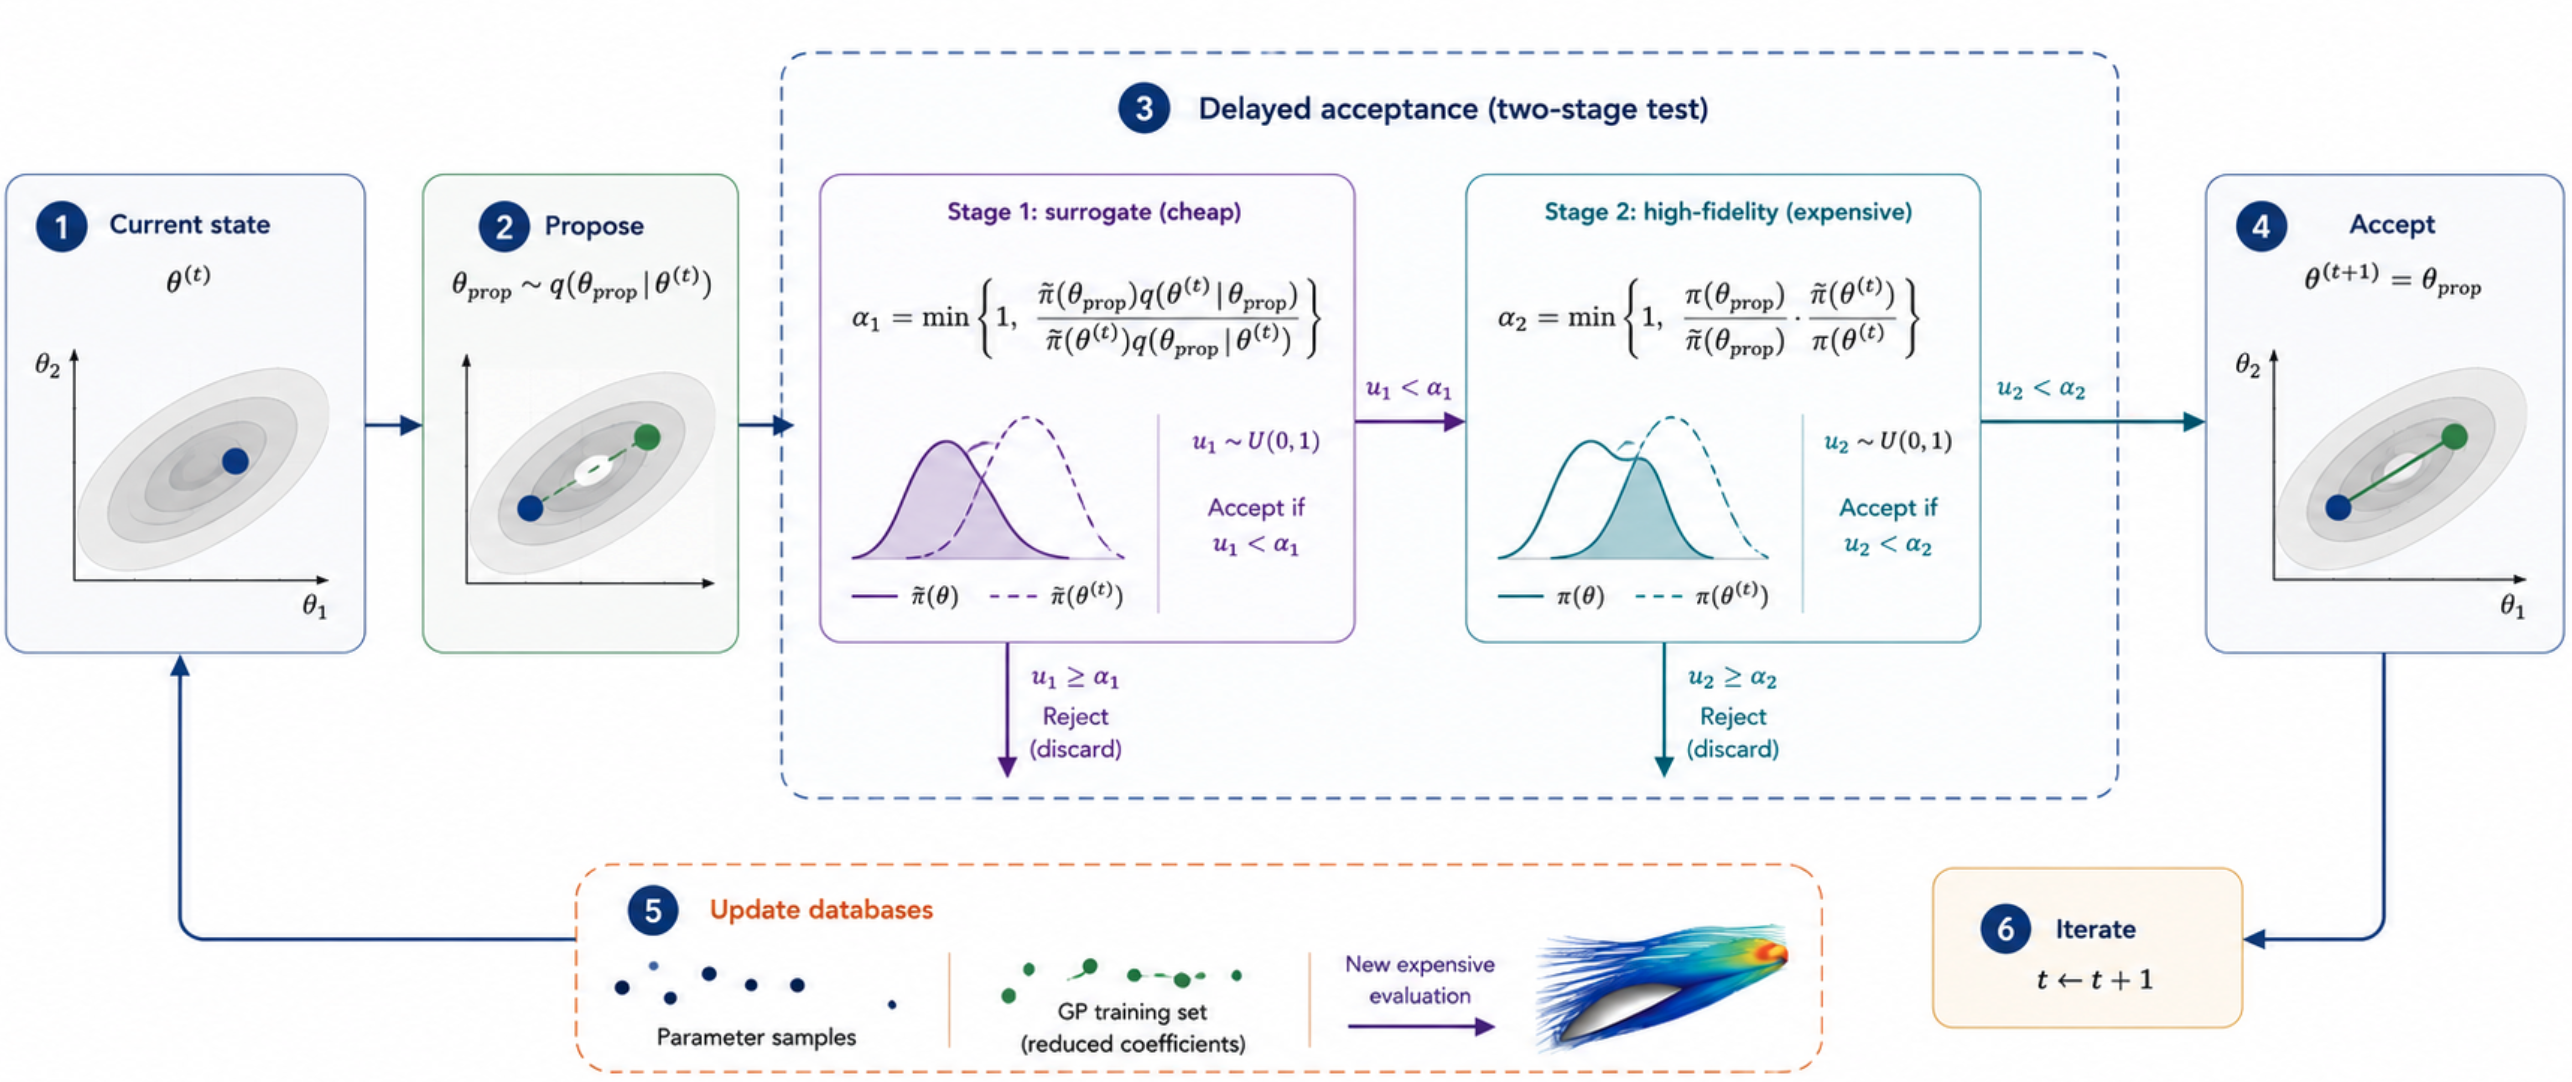
\includegraphics[width=\linewidth]{surrogate_mcmc.png}
    \caption{Placeholder: Simplified schematic of the proposed adaptive Surrogate Transition  framework. The uncertainty-aware POD–GP surrogate is used to construct an approximate likelihood for inexpensive first-stage acceptance decisions. During the adaptive phase, posterior-guided acquisition identifies new high-fidelity evaluations to enrich the surrogate, while the Surrogate Transition  subchain length is adjusted according to the estimated surrogate error. Once the surrogate satisfies the prescribed accuracy criterion, adaptation is terminated and the surrogate transition sampler proceeds with a fixed surrogate and transition kernel to generate posterior samples.}
    \label{fig:MCMC}
\end{figure}

The remainder of the paper is organized as follows. Section~\ref{sec:background} presents a background part on the Bayesian inverse problem and the delayed-acceptance construction.
Section~\ref{sec:methodology} presents the
POD-GP surrogate and its introduction in the sampling scheme. Section~\ref{sec:numerics} reports the numerical experiments on the benchmark problems.
Finally, Section~\ref{sec:conclusion} summarizes the
main findings and discusses possible extensions.

\section{Background and Motivation}
\label{sec:background}

In this section, we briefly recall the Bayesian formulation of inverse problems and the use of MCMC methods for posterior inference. We then introduce surrogate-based delayed-acceptance strategies for reducing the cost of repeated evaluations of expensive forward models. This also highlights the main limitation of standard fixed-surrogate approaches, namely that their performance depends on the surrogate being accurate in the posterior-relevant region. These observations motivate the adaptive framework developed in the next section.

\subsection{Bayesian inverse problem}
\label{sec:bayesian-background}

Inverse problems are concerned with inferring unknown properties of a system from indirect measurements or observational data through a mathematical model. These unknowns are represented by a parameter vector $\boldsymbol{\theta}\in\Theta\subset\mathbb R^n$, while the available observations are denoted by $\mathbf y_{\mathrm{obs}}\in\mathbb R^{d_y}$. We assume that parameters and observations are related through a high-fidelity forward map $\mathbf f_{\mathrm{HF}}:\Theta\to\mathbb R^{d_y}$ and an additive noise term, so that
\begin{equation}\label{eq:hf}
   \mathbf y_{\mathrm{obs}} = \mathbf f_{\mathrm{HF}}(\boldsymbol{\theta}) + \boldsymbol{\varepsilon}.
\end{equation}
In particular $\boldsymbol{\varepsilon}$ accounts for measurement noise and possible model discrepancy.

For a fixed $\boldsymbol{\theta}$, evaluating $\mathbf f_{\mathrm{HF}}(\boldsymbol{\theta})$ defines the corresponding forward problem, which, in many applications, requires the (expensive) solution of a Partial Differential Equation (PDE). The resulting observables may represent sensor measurements or more general quantities of interest derived from the PDE solution, such as spatial averages, fluxes, or derivatives. In this setting, $\boldsymbol{\theta}$ typically collects model coefficients, boundary conditions, or initial conditions characterizing the underlying physical system.

In the Bayesian setting, the unknown parameters are treated as random variables. The goal is to characterize the posterior distribution $\pi(\boldsymbol{\theta}\mid \mathbf y_{\mathrm{obs}})$ of the parameters given the observations $\mathbf y_{\mathrm{obs}}$. By Bayes' theorem,
\begin{equation}
\label{eq:bayes}
    \pi(\boldsymbol{\theta}\mid \mathbf y_{\mathrm{obs}})
    =
    \frac{\pi(\mathbf y_{\mathrm{obs}}\mid \boldsymbol{\theta})\,\pi(\boldsymbol{\theta})}
    {\pi(\mathbf y_{\mathrm{obs}})},
\end{equation}
where $\pi(\mathbf y_{\mathrm{obs}}\mid \boldsymbol{\theta})$ denotes the likelihood of the data given the parameters, $\pi(\boldsymbol{\theta})$ is the prior distribution encoding the available knowledge on $\boldsymbol{\theta}$ before observing the data, and $\pi(\mathbf y_{\mathrm{obs}})$ is the marginal distribution, or evidence, which acts as a normalizing constant and is given by
\begin{equation}
\label{eq:marginal}
    \pi(\mathbf y_{\mathrm{obs}})
    =
    \int_{\Theta}
    \pi(\mathbf y_{\mathrm{obs}}\mid \boldsymbol{\theta})\,\pi(\boldsymbol{\theta})
    \, d\boldsymbol{\theta}.
\end{equation}

The observation model induces a likelihood associated with the high-fidelity forward map. In general, if $\pi_{\varepsilon}$ denotes the probability density of the additive error $\boldsymbol{\varepsilon}$, then
\begin{equation}
\label{eq:hf-like-general}
    \pi(\mathbf y_{\mathrm{obs}}\mid \boldsymbol{\theta})
    =
    \pi_{\varepsilon}\!\left(
    \mathbf y_{\mathrm{obs}} - \mathbf f_{\mathrm{HF}}(\boldsymbol{\theta})
    \right).
\end{equation}
For simplicity, in the following we assume additive Gaussian noise, $\boldsymbol{\varepsilon}\sim\mathcal N(\mathbf 0,\mathbf \Gamma_{\mathrm{obs}})$, although the proposed methodology is not restricted to this setting. Under this assumption, the high-fidelity likelihood takes the form
\begin{equation}
\label{eq:hf-like-gaussian}
    \pi(\mathbf y_{\mathrm{obs}}\mid \boldsymbol{\theta})
    \propto
    \exp\!\left(
    -\frac{1}{2}
    \left\|
    \mathbf y_{\mathrm{obs}}-\mathbf f_{\mathrm{HF}}(\boldsymbol{\theta})
    \right\|^2_{\mathbf \Gamma_{\mathrm{obs}}^{-1}}
    \right).
\end{equation}

The evidence integral in \eqref{eq:marginal} cannot in general be evaluated analytically, and the posterior distribution is therefore not available in closed form. A standard strategy to explore such distributions is to resort to Markov chain Monte Carlo (MCMC) methods, which generate a Markov chain in the parameter space $\Theta$ having the posterior \eqref{eq:bayes} as invariant distribution. Among the available choices, the Metropolis--Hastings (MH) algorithm is one of the most widely used. Starting from a current state $\boldsymbol{\theta}$, MH generates a candidate $\boldsymbol{\theta}'$ from a proposal distribution $q(\cdot\mid\boldsymbol{\theta})$ and accepts it with probability
\begin{equation}
\label{eq:mh-acceptance}
    \alpha(\boldsymbol{\theta},\boldsymbol{\theta}')
    =
    \min\left\{
    1,
    \frac{
    \pi(\mathbf y_{\mathrm{obs}}\mid \boldsymbol{\theta}')\,
    \pi(\boldsymbol{\theta}')\,
    q(\boldsymbol{\theta}\mid\boldsymbol{\theta}')
    }{
    \pi(\mathbf y_{\mathrm{obs}}\mid \boldsymbol{\theta})\,
    \pi(\boldsymbol{\theta})\,
    q(\boldsymbol{\theta}'\mid\boldsymbol{\theta})
    }
    \right\}.
\end{equation}
While this avoids the explicit computation of the evidence, each MH step still requires one evaluation of the high-fidelity likelihood, and hence one solve of the expensive forward model. The full procedure is summarized in Algorithm~\ref{alg:mh}. 

A comprehensive exploration of the posterior distribution typically requires a large number of MCMC iterations, as MH algorithm usually exhibits frequent rejections and strong correlation between successive samples, making the overall procedure computationally prohibitive. This motivates the introduction of surrogate-based strategies aimed at reducing the number of high-fidelity model evaluations while preserving the high-fidelity posterior as the target distribution.


\begin{algorithm}[t]
\caption{Metropolis--Hastings (MH)}
\label{alg:mh}
\begin{algorithmic}[1]
\Statex \textbf{Input:} Likelihood $\pi(\mathbf y_{\mathrm{obs}}\mid \cdot)$, prior distribution $\pi(\cdot)$, proposal distribution $q(\cdot\mid\cdot)$, initial sample $\boldsymbol{\theta}^{(0)}$, number of samples $N$
\Statex \textbf{Output:} Chain of samples $\{\boldsymbol{\theta}^{(j)}\}_{j=1}^N$
\For{$j=1,\dots,N$}
    \State Propose $\boldsymbol{\theta}' \sim q(\cdot\mid \boldsymbol{\theta}^{(j-1)})$
    \State Compute the acceptance probability
    \begin{equation*}
        \alpha\!\left(\boldsymbol{\theta}^{(j-1)},\boldsymbol{\theta}'\right)
        =
        \min\left\{
        1,
        \frac{
        \pi(\mathbf y_{\mathrm{obs}}\mid \boldsymbol{\theta}')\,
        \pi(\boldsymbol{\theta}')\,
        q(\boldsymbol{\theta}^{(j-1)}\mid \boldsymbol{\theta}')
        }{
        \pi(\mathbf y_{\mathrm{obs}}\mid \boldsymbol{\theta}^{(j-1)})\,
        \pi(\boldsymbol{\theta}^{(j-1)})\,
        q(\boldsymbol{\theta}'\mid \boldsymbol{\theta}^{(j-1)})
        }
        \right\}
    \end{equation*}
    \State Accept $\boldsymbol{\theta}'$ with probability $\alpha$; if accepted set $\boldsymbol{\theta}^{(j)}=\boldsymbol{\theta}'$, otherwise set $\boldsymbol{\theta}^{(j)}=\boldsymbol{\theta}^{(j-1)}$
\EndFor
\end{algorithmic}
\end{algorithm}

\subsection{Delayed-acceptance MCMC}
\label{sec:da-background}

In many applications, it is possible to replace the high fidelity model in \eqref{eq:hf} with a cheap approximation $\mathbf{f}_{\mathrm{LF}}\approx \mathbf{f}_{\mathrm{HF}}$. Replacing $\mathbf{f}_{\mathrm{HF}}$ with $\mathbf{f}_{\mathrm{LF}}$ in the observation model induces the low-fidelity likelihood
\begin{equation}
\label{eq:lf-like-general}
\pi_{\mathrm{LF}}(\mathbf y_{\mathrm{obs}}\mid \boldsymbol{\theta})
=
\pi_{\varepsilon}\left(
\mathbf y_{\mathrm{obs}}-\mathbf f_{\mathrm{LF}}(\boldsymbol{\theta})
\right),
\end{equation}
which provides a computationally inexpensive approximation to the high-fidelity likelihood. When the surrogate model is sufficiently accurate, it may be used directly within an MH scheme to sample from an approximate posterior distribution. In general, however, constructing a sufficiently accurate surrogate over the entire parameter space may be computationally prohibitive, particularly for high-dimensional or strongly nonlinear forward models. Moreover, since the posterior often concentrates on a relatively small region of the parameter space, global surrogate accuracy is neither necessary nor necessarily the most efficient objective \cite{LiMarzouk2014}. The errors in the surrogate forward model propagate through the likelihood and lead to discrepancies between the approximate and high-fidelity posterior distributions \cite{CotterDashtiStuart2010}.

The idea underlying Delayed-Acceptance (DA) MCMC is to find a trade-off between computational efficiency of the approximation and accuracy of the high-fidelity target. In particular, the surrogate likelihood is used as an initial screening mechanism, and only proposals that pass this first stage are subsequently evaluated using the high-fidelity likelihood. In this way, expensive high-fidelity model evaluations are restricted to candidates that are deemed sufficiently promising by the surrogate.

More precisely, let $
\label{eq:lf-posterior}
\pi_{\mathrm{LF}}(\boldsymbol{\theta}\mid\mathbf y_{\mathrm{obs}})
\propto
\pi_{\mathrm{LF}}(\mathbf y_{\mathrm{obs}}\mid\boldsymbol{\theta})
\pi(\boldsymbol{\theta}) $
denote the approximate posterior induced by the low-fidelity likelihood. Starting from the current state $\boldsymbol{\theta}$, a fixed-length MH subchain of L steps is first simulated targeting $\pi_{\mathrm{LF}}(\boldsymbol{\theta}\mid\mathbf y_{\mathrm{obs}})$. The final state of this subchain, denoted by $\boldsymbol{\theta}'$, is then used as a candidate for the high-fidelity chain and is accepted with probability
\begin{equation}
\label{eq:da-acceptance}
\alpha_{\mathrm{DA}}(\boldsymbol{\theta},\boldsymbol{\theta}’)
=
\min\left\{
1,
\frac{
\pi(\mathbf y_{\mathrm{obs}}\mid\boldsymbol{\theta}’)
\pi_{\mathrm{LF}}(\mathbf y_{\mathrm{obs}}\mid\boldsymbol{\theta})
}{
\pi(\mathbf y_{\mathrm{obs}}\mid\boldsymbol{\theta})
\pi_{\mathrm{LF}}(\mathbf y_{\mathrm{obs}}\mid\boldsymbol{\theta}’)
}
\right\}.
\end{equation}
It is possible to show that, despite using the surrogate model to generate candidates, the resulting Markov chain preserves the high-fidelity posterior as its invariant distribution.

\begin{algorithm}[t]
\caption{Delayed-acceptance MCMC (DA)}
\label{alg:da}
\begin{algorithmic}[1]
\Statex \textbf{Input:}
High-fidelity likelihood $\pi(\mathbf y_{\mathrm{obs}}\mid\cdot)$,
low-fidelity likelihood $\pi_{\mathrm{LF}}(\mathbf y_{\mathrm{obs}}\mid\cdot)$,
prior distribution $\pi(\cdot)$,
proposal distribution $q(\cdot\mid\cdot)$,
initial sample $\boldsymbol{\theta}^{(0)}$,
subchain length $L$,
number of samples $N$
\Statex \textbf{Output:}
Chain of samples $\{\boldsymbol{\theta}^{(j)}\}_{j=1}^N$

\For{$j=1,\dots,N$}

    \State Starting from $\boldsymbol{\theta}^{(j-1)}$, generate an
    $L$-step low-fidelity MH subchain using Algorithm~\ref{alg:mh}:
    \begin{equation*}
        \left\{
        \boldsymbol{\vartheta}^{(\ell)}
        \right\}_{\ell=1}^{L}
        =
        \operatorname{MH}\!\left(
        \pi_{\mathrm{LF}}(\mathbf y_{\mathrm{obs}}\mid\cdot),
        \pi(\cdot),
        q(\cdot\mid\cdot),
        \boldsymbol{\theta}^{(j-1)},
        L
        \right)
    \end{equation*}

    \State Set the candidate
    $\boldsymbol{\theta}'=\boldsymbol{\vartheta}^{(L)}$

    \State Compute the delayed-acceptance probability
    \begin{equation*}
    \alpha_{\mathrm{DA}}
    \!\left(
    \boldsymbol{\theta}^{(j-1)},
    \boldsymbol{\theta}'
    \right)
    =
    \min\left\{
    1,
    \frac{
    \pi(
    \mathbf y_{\mathrm{obs}}
    \mid
    \boldsymbol{\theta}'
    )\,
    \pi_{\mathrm{LF}}(
    \mathbf y_{\mathrm{obs}}
    \mid
    \boldsymbol{\theta}^{(j-1)}
    )
    }{
    \pi(
    \mathbf y_{\mathrm{obs}}
    \mid
    \boldsymbol{\theta}^{(j-1)}
    )\,
    \pi_{\mathrm{LF}}(
    \mathbf y_{\mathrm{obs}}
    \mid
    \boldsymbol{\theta}'
    )
    }
    \right\}
    \end{equation*}

    \State Accept $\boldsymbol{\theta}'$ with probability
    $\alpha_{\mathrm{DA}}$; if accepted set
    $\boldsymbol{\theta}^{(j)}=\boldsymbol{\theta}'$,
    otherwise set
    $\boldsymbol{\theta}^{(j)}
    =\boldsymbol{\theta}^{(j-1)}$

\EndFor
\end{algorithmic}
\end{algorithm}

When the surrogate provides a sufficiently accurate representation of the high-fidelity target, DA can yield substantial computational gains by reducing the number of expensive model evaluations while improving mixing of the chain. In particular, the use of inexpensive low-fidelity subchains can increase the effective sample size obtained for a given computational budget. Conversely, when the surrogate poorly represents the high-fidelity posterior, candidates generated at the low-fidelity level may be frequently rejected by the high-fidelity correction, leading to low acceptance rates, increased self-correlation, and poor overall sampling efficiency. The performance of DA scheme therefore remains strongly dependent on the quality of the surrogate approximation.

This limitation has motivated adaptive approaches in which information acquired during sampling is used to improve the approximation in posterior-relevant regions or to correct discrepancies between low- and high-fidelity models \cite{lykkegaard23}. The approach developed in this work follows this general motivation, but adopts a different strategy: the surrogate is refined online as sampling proceeds, while its predictive uncertainty is incorporated into the inference procedure to prevent unreliable surrogate predictions from influencing the exploration of the posterior.

\section{Methodology}
\label{sec:methodology}

The proposed method embeds a probabilistic reduced-order surrogate within a
delayed-acceptance MCMC framework. The low-fidelity model combines Proper
Orthogonal Decomposition (POD) and Gaussian Process (GP) regression. POD
provides a low-dimensional representation of the high-fidelity model output,
whereas GP regression approximates the dependence of the reduced coefficients
on the model parameters. The resulting POD–GP surrogate provides both a
predictive mean and a predictive covariance in the observation space.

Compared with a standard delayed-acceptance scheme based on a deterministic
surrogate, the probabilistic formulation offers two main advantages:
\begin{itemize}
\item Uncertainty-aware likelihood:
the surrogate predictive covariance is incorporated into the
low-fidelity likelihood by inflating the observation-noise covariance.
The resulting likelihood therefore accounts not only for measurement
uncertainty, but also for the uncertainty associated with the surrogate
approximation. Ideally, predictions in poorly resolved regions are
assigned a larger effective covariance, reducing the risk that surrogate
errors drift the exploration of the parameter space.

\item Online surrogate enrichment:
the predictive uncertainty also provides a criterion for identifying
parameter values at which the surrogate should be refined. Whenever the
uncertainty at a sampled parameter exceeds a prescribed threshold, the
high-fidelity model is evaluated and the resulting parameter-output pair
is added to the training set. GP regression is particularly well suited to
this sequential setting, since newly acquired observations can be used to
update the approximation as sampling proceeds. In this way,
high-fidelity evaluations generated during posterior exploration are
reused to improve the surrogate in posterior-relevant regions, allowing
the algorithm to rely progressively more on the low-fidelity model.

\end{itemize}

Surrogate adaptation is performed during an initial adaptive phase. In the
same phase, the high-fidelity evaluations carried out at the correction stage
of the delayed-acceptance algorithm are used to monitor the discrepancy
between the low- and high-fidelity predictions. This discrepancy determines
the length of the low-fidelity subchain: the subchain is shortened when the
surrogate error is large and lengthened when the surrogate provides a
sufficiently accurate approximation.

The adaptive phase is used exclusively to construct and calibrate the
surrogate and to determine the correction schedule. In a second phase,
both the surrogate and the subchain length are kept fixed.
The resulting sampler is therefore a standard delayed-acceptance Markov chain
with a fixed low-fidelity model and a high-fidelity correction step, and hence
preserves the high-fidelity posterior as its invariant distribution.

\subsection{Surrogate definition and approximate likelihood}
The delayed-acceptance algorithm requires a cheapapproximation of the high-fidelity parameter-to-observable map $\mathbf{f}_{\mathrm{HF}}:\Theta\rightarrow\mathbb{R}^{d_y}$.
To this end, we combine POD with GP regression. POD is first used to construct a low-dimensional representation of the model outputs, after which GP regression is employed to approximate the mapping between the parameter vector and the reduced coordinates. This substantially reduces the complexity of the regression problem while retaining the dominant features of the high-fidelity solutions.
\subsubsection{Proper Orthogonal Decomposition}

Let $
\mathcal D
=
\left\{
\left(
\boldsymbol{\theta}^{(i)},
\mathbf f_{\mathrm{HF}}(\boldsymbol{\theta}^{(i)})
\right)
\right\}_{i=1}^{N_s} $
denote an offline available dataset of input - (high fidelity) output pairs. Assuming the snapshots have been centered (i.e. removing the mean), the snapshot matrix is defined as
\begin{equation}
\mathbf{S}
=
\left[
\begin{array}{ccc}
| & & | \\
\mathbf{f}_{\mathrm{HF}}\!\left(\boldsymbol{\theta}^{(1)}\right)
& \cdots &
\mathbf{f}_{\mathrm{HF}}\!\left(\boldsymbol{\theta}^{(N_s)}\right)\\
| & & |
\end{array}
\right]
\in \mathbb{R}^{d_y \times N_s}.
\end{equation}
We then perform the singular value decomposition of the snapshot matrix:
\begin{equation}
\mathbf S
=
\mathbf U
\boldsymbol{\Sigma}
\mathbf V^{\top}.
\end{equation}
The resulting POD basis on the full grid is
\begin{equation}
\mathbf\Phi
=
[\mathbf u_1,\ldots,\mathbf u_r],
\end{equation}
which is formed by retaining the first \(r\) left singular vectors, where \(r\) is chosen such that
\begin{equation}
\frac{\sum_{i=1}^{r}\sigma_i^2}
{\sum_i\sigma_i^2}
\geq
0.95.
\end{equation}

For a new high fidelity solution we can then obtain its reduced dimension representiation thorugh the projection operator $\boldsymbol{\Phi}$:
\begin{equation}
\mathbf c(\boldsymbol{\theta})
=
\mathbf\Phi^{\top}
\mathbf f_{\mathrm{HF}}(\boldsymbol{\theta}).
\end{equation}
At the same time, given the reduced representation, the high fidelity solution is approximated by re-projecting onto the full space:
The high-fidelity solution is approximated by
\begin{equation}
\mathbf f_{\mathrm{HF}}(\boldsymbol{\theta})
\approx
\mathbf\Phi\,\mathbf c(\boldsymbol{\theta}).
\end{equation}
The remaining task is therefore to approximate the nonlinear mapping
$
\boldsymbol{\theta}
\longmapsto
\mathbf c(\boldsymbol{\theta}),
$
which is achieved using Gaussian Process regression.

\subsubsection{Gaussian Process Regression}
Let $
\mathcal D_{\mathrm{GP}}
=
\left\{
\left(
\boldsymbol{\theta}^{(i)},
\mathbf c^{(i)}
\right)
\right\}_{i=1}^{N_{\mathrm{GP}}},
$
denote the available training set, where the reduced coefficients
\(\mathbf c^{(i)}\) are obtained by projecting the corresponding
high-fidelity solutions onto the POD basis. Note that $N_{GP} \neq N_s$ in general and we will describe in the overall algorithm how these data are obtained.
Each POD coefficient is approximated independently using GP 
regression. For the \(j\)-th coefficient, we assume the prior
\begin{equation}
c_j(\boldsymbol{\theta})
\sim
\mathcal{GP}
\left(
0,
k_{\mathbf w}
(\boldsymbol{\theta},\boldsymbol{\theta}')
\right),
\end{equation}
where \(k_{\mathbf w}\) is a parametric covariance kernel with
hyperparameters \(\mathbf w\). In this work, standard kernels such as the
squared exponential or Matérn covariance functions may be employed.
Conditioning on \(\mathcal D_{\mathrm{GP}}\), the predictive distribution at
\(\boldsymbol{\theta}\) is
\begin{equation}
c_j(\boldsymbol{\theta})
\mid
\mathcal D_{\mathrm{GP}}
\sim
\mathcal N
\left(
\widehat c_j(\boldsymbol{\theta}),
s_j^2(\boldsymbol{\theta})
\right),
\end{equation}
with predictive mean and variance
\begin{align}
\widehat c_j(\boldsymbol{\theta})
&=
\mathbf k_{\mathbf w}(\boldsymbol{\theta})^\top
\mathbf K_{\mathbf w}^{-1}
\mathbf c_j,
\\
s_j^2(\boldsymbol{\theta})
&=
k_{\mathbf w}(\boldsymbol{\theta},\boldsymbol{\theta})
-
\mathbf k_{\mathbf w}(\boldsymbol{\theta})^\top
\mathbf K_{\mathbf w}^{-1}
\mathbf k_{\mathbf w}(\boldsymbol{\theta}).
\end{align}
Here,
\(\mathbf K_{\mathbf w}\in
\mathbb R^{N_{\mathrm{GP}}\times N_{\mathrm{GP}}}\) is the covariance matrix
with entries
\begin{equation}
[\mathbf K_{\mathbf w}]_{mn}
=
k_{\mathbf w}
\left(
\boldsymbol{\theta}^{(m)},
\boldsymbol{\theta}^{(n)}
\right),
\end{equation}
and
\begin{equation}
\mathbf k_{\mathbf w}(\boldsymbol{\theta})
=
\left[
k_{\mathbf w}(\boldsymbol{\theta},\boldsymbol{\theta}^{(1)}),
\ldots,
k_{\mathbf w}(\boldsymbol{\theta},\boldsymbol{\theta}^{(N_{\mathrm{GP}})})
\right]^\top.
\end{equation}
Moreover,
\begin{equation}
\mathbf c_j
=
\left[
c_j^{(1)},
\ldots,
c_j^{(N_{\mathrm{GP}})}
\right]^\top
\end{equation}
collects the training values of the \(j\)-th POD coefficient.

Since the POD basis decorrelates the reduced coefficients, each coefficient is modeled independently by a scalar Gaussian process. This avoids the need for a multi-output Gaussian process while retaining the dominant variability of the solution. We thus have:
\begin{equation}
\widehat{\mathbf c}(\boldsymbol{\theta})
=
\left[
\widehat c_1(\boldsymbol{\theta}),
\ldots,
\widehat c_r(\boldsymbol{\theta})
\right]^T,
\end{equation}
while the corresponding covariance matrix is
\begin{equation}
\mathbf\Sigma_c(\boldsymbol{\theta})
=
\operatorname{diag}
\left(
s_1^2(\boldsymbol{\theta}),
\ldots,
s_r^2(\boldsymbol{\theta})
\right).
\end{equation}
The surrogate prediction of the high-fidelity model, comprising both the mean and the predictive variance, is therefore obtained by projecting the two reduced quantities on the full space:
\begin{align}
\mathbf f_{\mathrm{LF}}(\boldsymbol{\theta})
=
\mathbf\Phi
\widehat{\mathbf c}(\boldsymbol{\theta}) \in \mathbb{R}^{d_y},
\qquad
\mathbf\Sigma_{\mathrm{LF}}(\boldsymbol{\theta})
=
\mathbf\Phi
\mathbf\Sigma_c(\boldsymbol{\theta})
\mathbf\Phi^T. \in \mathbb{R}^{d_y\times d_y}
\end{align}
Assuming additive Gaussian observation noise and independent Gaussian surrogate
errors, the predictive distribution of the observations remains Gaussian, with
covariance given by the sum of the observation covariance
\(\mathbf{\Gamma}_{\mathrm{obs}}\) and the surrogate predictive covariance
\(\mathbf{\Sigma}_{\mathrm{LF}}(\boldsymbol{\theta})\). The resulting
approximate likelihood is
\begin{equation}
\pi_{\text{LF}}(\mathbf y_{\mathrm{obs}}\mid\boldsymbol{\theta})
\propto
\left|
\mathbf\Gamma_{\mathrm{obs}}
+
\mathbf\Sigma_{\mathrm{LF}}(\boldsymbol{\theta})
\right|^{-1/2}
\exp\!\left(
-\frac12
\left\|
\mathbf y_{\mathrm{obs}}
-
\mathbf f_{\mathrm{LF}}(\boldsymbol{\theta})
\right\|^2_{
(\mathbf\Gamma_{\mathrm{obs}}
+
\mathbf\Sigma_{\mathrm{LF}}(\boldsymbol{\theta}))^{-1}
}
\right).
\end{equation}
More generally, for non-Gaussian likelihoods, the surrogate uncertainty can be
incorporated by marginalizing the likelihood with respect to the surrogate
predictive distribution. An simplified scheme of the surrogate construction and usage is presented in Fig. \ref{fig:surr}.
\begin{figure}
    \centering
    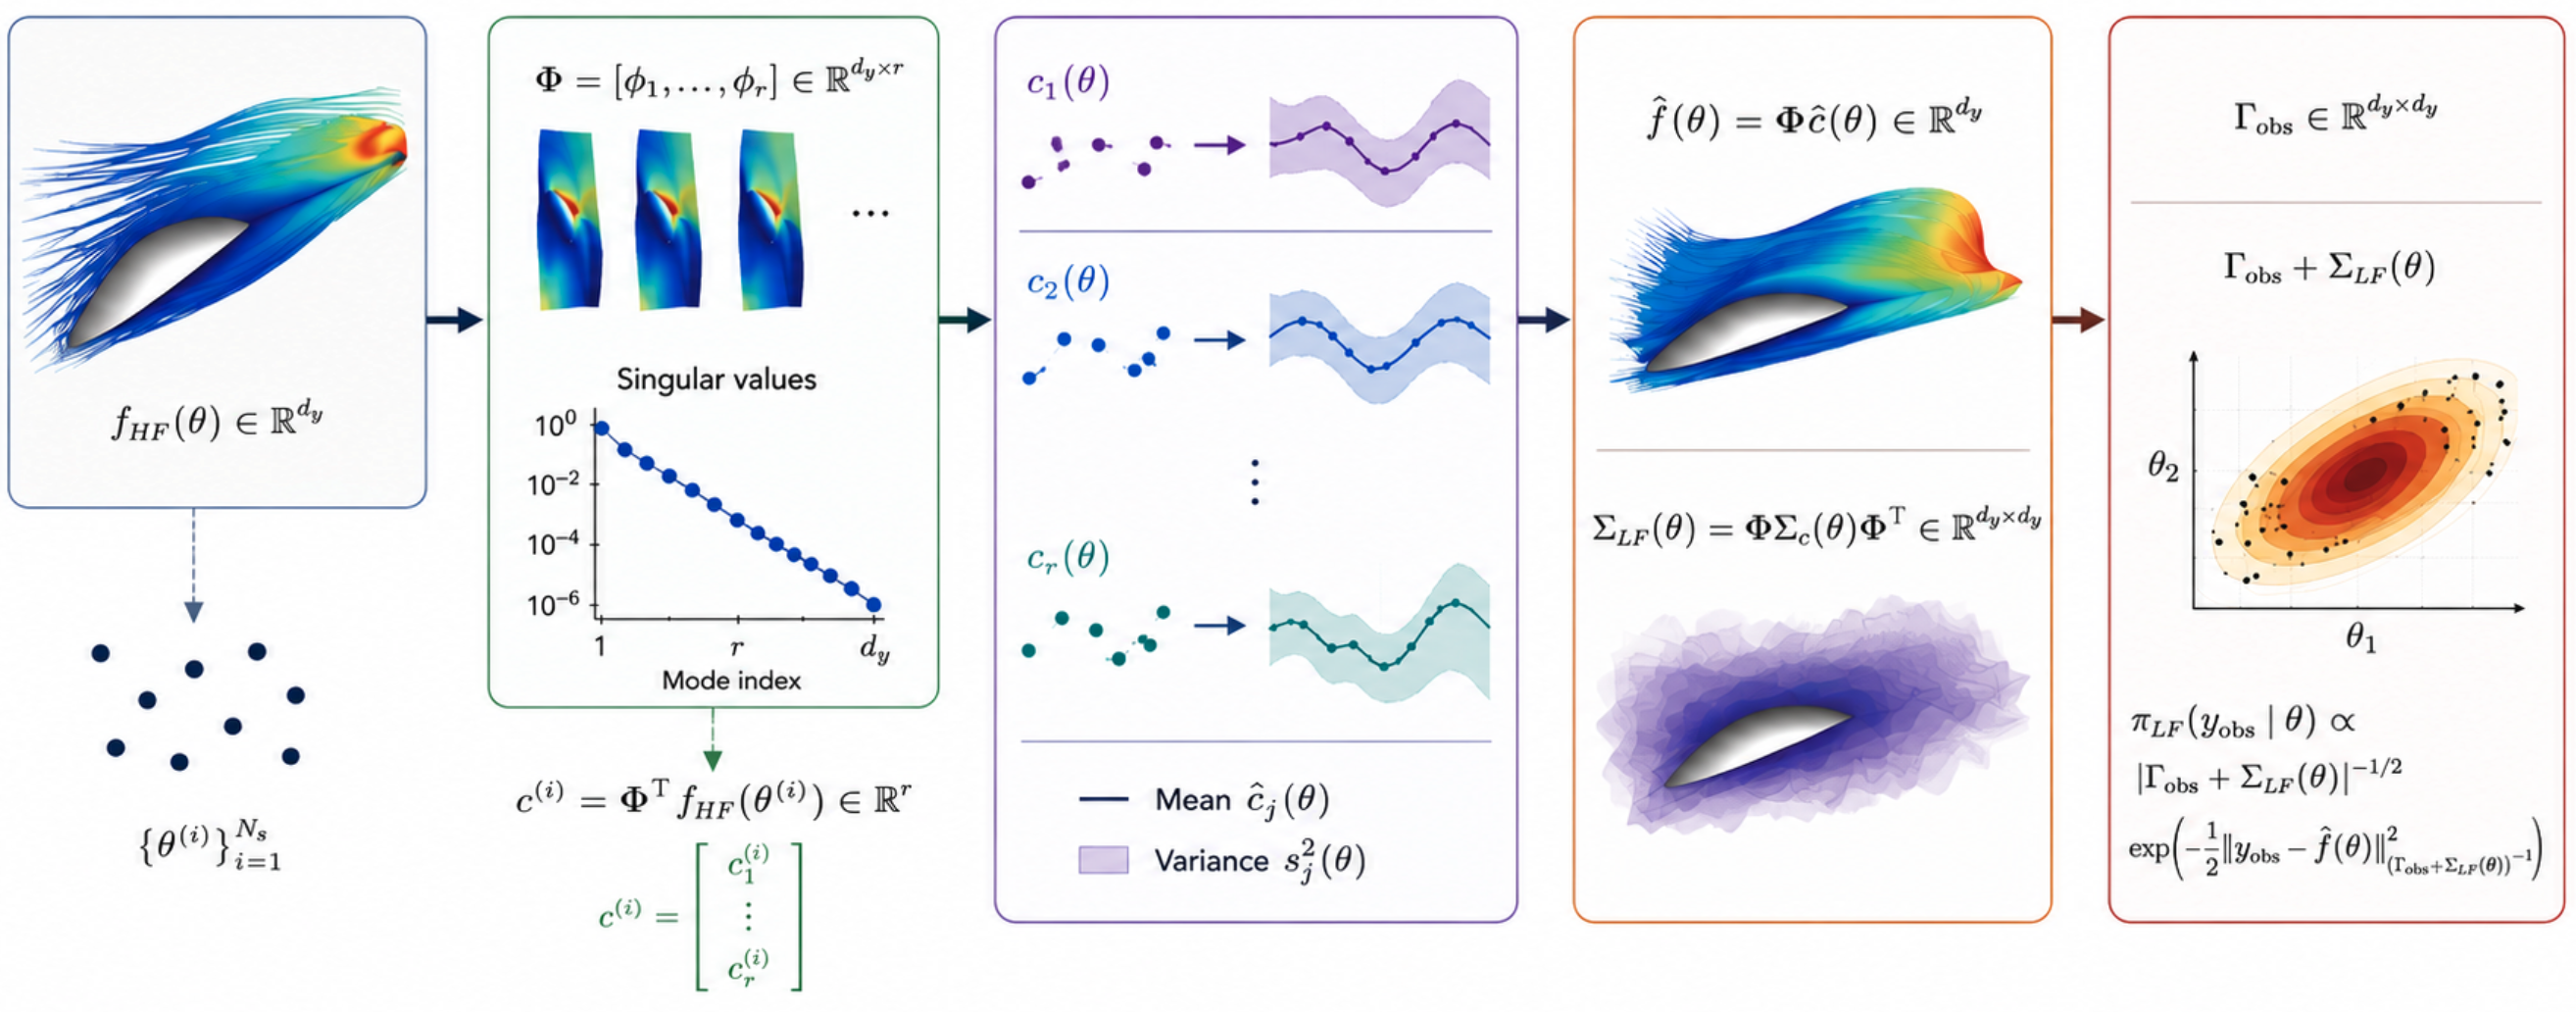
\includegraphics[width=0.9\linewidth]{surrogate_graphical.png}
    \caption{GPT-Place holder. Simplified schematic of the LF model used to construct the approximate likelihood. The surrogate combines POD for dimensionality reduction with GP regression to predict the reduced coefficients. The GP predictive uncertainty is first estimated in the reduced space and then propagated to the full observation space, and is then incorporated into the approximate likelihood.}
    \label{fig:surr}
\end{figure}

\subsection{Adaptive sampling scheme}

The surrogate model introduced above is embedded within an adaptive delayed-acceptance framework consisting of three stages:

\begin{itemize}
    \item \textbf{Offline stage:} an initial training set is constructed by drawing $N_s$ parameter samples from the prior distribution using a space-filling design, such as Latin Hypercube Sampling. The corresponding high-fidelity evaluations are used to construct the POD basis $\mathbf{\Phi}$ and to initialize the GP training set
    $\mathcal{D}_{\mathrm{GP}}^{(0)}$, yielding the initial surrogate
    $\mathbf{f}_{\mathrm{LF}}^{(0)}$ and the corresponding approximate likelihood
    $\pi_{\mathrm{LF}}^{(0)}$.

    \item \textbf{Adaptive online stage:} posterior sampling is performed using delayed-acceptance MCMC initialized with the surrogate likelihood
    $\pi_{\mathrm{LF}}^{(0)}$ and an initial subchain length $L^{(0)}$. During this stage, the surrogate is iteratively enriched by incorporating new high-fidelity evaluations selected according to the adaptive strategy described below. The subchain length is updated simultaneously to account for the evolving surrogate accuracy. At adaptive iteration $j$, the algorithm is characterized by the GP training set $\mathcal{D}_{\mathrm{GP}}^{(j)}$, the surrogate $\mathbf{f}_{\mathrm{LF}}^{(j)}$, the approximate likelihood $\pi_{\mathrm{LF}}^{(j)}$, and the subchain length $L^{(j)}$. The adaptation is performed for at most $N_{\mathrm{adapt}}$ iterations or until the prescribed stopping criterion is satisfied.

    \item \textbf{Fixed-kernel online stage:} once adaptation is terminated, both the surrogate and the subchain length are frozen. The delayed-acceptance sampler is then continued using the fixed approximate likelihood
    $\pi_{\mathrm{LF}}^{(N_{\mathrm{adapt}})}$ and subchain length
    $L^{(N_{\mathrm{adapt}})}$, thereby defining a fixed transition kernel for posterior sampling and guaranteeing sampling from the true posterior.
\end{itemize}
For what concerns the surrogate likelihood, at a candidate parameter value $\boldsymbol{\theta}$, the surrogate provides the predictive mean
$\mathbf{f}_{\mathrm{LF}}^{(j)}(\boldsymbol{\theta})$ and predictive variance
$\boldsymbol{\sigma}_{\mathrm{LF}}^{2,(j)}(\boldsymbol{\theta})$. A high-fidelity evaluation is triggered whenever the average predictive variance satisfies
\begin{equation}
    \frac{1}{d_y}
    \sum_{i=1}^{d_y}
    \sigma_{\mathrm{LF},i}^{2,(j)}(\boldsymbol{\theta})
    >
    \gamma^2,
\end{equation}
where $\gamma$ is a prescribed uncertainty threshold. The resulting pair
$(\boldsymbol{\theta},\mathbf{f}_{\mathrm{HF}}(\boldsymbol{\theta}))$
is added to $\mathcal{D}_{\mathrm{GP}}^{(j)}$, and the GP surrogate is updated. High-fidelity evaluations required by the second delayed-acceptance stage are also incorporated into the training set in the same manner.

The subchain length is adapted using the discrepancy between the surrogate prediction, evaluated before enrichment, and the corresponding high-fidelity output. Specifically, at the $k$-th high-fidelity evaluation, the error is measured as
\begin{equation}
    e_k
    =
    \left[
    \frac{1}{d_y}
    \left\|
    \mathbf{f}_{\mathrm{HF}}(\boldsymbol{\theta}_k)
    -
    \mathbf{f}_{\mathrm{LF}}^{(j)}(\boldsymbol{\theta}_k)
    \right\|_2^2
    \right]^{1/2}.
\end{equation}
After every $N_L$ high-fidelity evaluations, the subchain length is updated according to
\begin{equation}
    L^{(j+1)}
    =
    \begin{cases}
        \max\!\left\{L_{\min},
        \left\lfloor \rho_- L^{(j)}\right\rfloor\right\},
        & e_k>\varepsilon_L, \\[1mm]
        \min\!\left\{L_{\max},
        \left\lceil \rho_+ L^{(j)}\right\rceil\right\},
        & e_k\leq\varepsilon_L,
    \end{cases}
\end{equation}
where $\varepsilon_L$ is the target surrogate error,
$0<\rho_-<1$ and $\rho_+>1$ are contraction and expansion factors, and
$L_{\min}$ and $L_{\max}$ prescribe admissible bounds. Hence, inaccurate surrogate predictions lead to more frequent high-fidelity corrections, whereas sufficiently accurate predictions allow longer surrogate subchains.

The adaptive stage is terminated when the surrogate error remains below the prescribed tolerance for a specified number of consecutive updates, or when the maximum number of adaptive iterations, $N_{\mathrm{adapt}}$, is reached. The surrogate model and the subchain length obtained at termination are then fixed for the final delayed-acceptance sampling stage.

\begin{algorithm}[t]
\caption{Adaptive delayed-acceptance sampling scheme}
\label{alg:adaptive_da}
\begin{algorithmic}[1]
\Statex \textbf{Input:} Initial design size $N_s$, initial subchain length $L^{(0)}$,
maximum number of adaptive blocks $N_{\mathrm{adapt}}$, adaptive block size
$N_b$, and final sampling length $N_{\mathrm{final}}$
\Statex \textbf{Output:} Fixed-kernel posterior chain
$\{\boldsymbol{\theta}^{(n)}\}_{n=1}^{N_{\mathrm{final}}}$
\Statex
\Statex{\textbf{Offline Stage:}}

\State Draw $\{\boldsymbol{\theta}^{(i)}\}_{i=1}^{N_s}$ from the prior using
a space-filling design and evaluate $\mathbf f_{\mathrm{HF}}$
\State Construct the POD basis $\mathbf\Phi$ and initialize
$\mathcal D_{\mathrm{GP}}^{(0)}$
\State Train the initial surrogate and define
$\pi_{\mathrm{LF}}^{(0)}$
\Statex
\Statex{\textbf{Adaptive Online Stage:}}
\State Initialize the chain state $\boldsymbol{\theta}^{(0)}$ and set $j=0$
\While{$j<N_{\mathrm{adapt}}$ and the adaptive stopping criterion is not satisfied}
    \State Run an $N_b$-step delayed-acceptance block using
    Algorithm~\ref{alg:da}, with fixed
    $\pi_{\mathrm{LF}}^{(j)}$ and $L^{(j)}$
    \State Collect the high-fidelity evaluations generated by the
    delayed-acceptance corrections
    \State Select additional enrichment points for which
    \[
        \frac{1}{d_y}
        \operatorname{tr}
        \!\left(
        \mathbf\Sigma_{\mathrm{LF}}^{(j)}
        (\boldsymbol{\theta})
        \right)
        > \gamma^2
    \]
    and evaluate $\mathbf f_{\mathrm{HF}}$ at these points
    \State Form $\mathcal D_{\mathrm{GP}}^{(j+1)}$ by augmenting
    $\mathcal D_{\mathrm{GP}}^{(j)}$ with the newly acquired data
    \State Compute the surrogate discrepancies at the newly evaluated
    high-fidelity points
    \State Retrain the GP surrogate and define
    $\pi_{\mathrm{LF}}^{(j+1)}$
    \State Update $L^{(j+1)}$ according to the error-based adaptation rule
    \State Set $j\gets j+1$
\EndWhile
\Statex
\Statex{\textbf{Fixed Kernel Online Stage:}}
\State Freeze the surrogate likelihood
$\pi_{\mathrm{LF}}^\star=\pi_{\mathrm{LF}}^{(j)}$
and the subchain length $L^\star=L^{(j)}$
\State Generate the final chain by applying Algorithm~\ref{alg:da} with
$\pi_{\mathrm{LF}}^\star$, $L^\star$, and
$N=N_{\mathrm{final}}$:
    \begin{equation*}
        \left\{
        \boldsymbol{\theta}^{(n)}
        \right\}_{n=1}^{N_{final}}
        =
        \operatorname{DA}\!\left(
        \pi(\mathbf y_{\mathrm{obs}}\mid\cdot),
        \pi_{\mathrm{LF}}^{\star}(\mathbf y_{\mathrm{obs}}\mid\cdot),
        \pi(\cdot),
        q(\cdot\mid\cdot),
        \boldsymbol{\theta}^{(j-1)},
        L^\star,
        N_{\text{final}}
        \right)
    \end{equation*}
\end{algorithmic}
\end{algorithm}

\section{Results}\label{sec:numerics}
\section{Conclusion}\label{sec:conclusion}


\bibliographystyle{elsarticle-num}
\bibliography{references}

\end{document}
